% ============================================================================
% Evidence-Bounded CAD Repair for Simulation Meshing
% Hexera CAD Repair System - technical white paper
%
% Overleaf: upload this file (and refs.bib), set the compiler to pdfLaTeX,
% and set main.tex as the main document. Two passes resolve the references.
% Every figure quoted here comes from a committed evidence README under
% devtools/validation/evidence/ or from docs/superpowers/specs/; update the
% paper with the evidence, never ahead of it.
% ============================================================================
\documentclass[11pt,onecolumn]{article}

\usepackage[T1]{fontenc}
\usepackage[utf8]{inputenc}
\usepackage{charter}                 % serif text face; mathdesign/utopia also fine
\usepackage[scaled=0.86]{beramono}   % mono for code, sized to sit with Charter
\usepackage[letterpaper,margin=1in]{geometry}
\usepackage{microtype}
\setlength{\emergencystretch}{1.2em}
\usepackage{booktabs}
\usepackage{tabularx}
\usepackage{array}
\usepackage{graphicx}
\usepackage{amsmath,amssymb}
\usepackage{algorithm}
\usepackage{algpseudocode}
\usepackage{float}
\usepackage{tikz}
\usetikzlibrary{arrows.meta,positioning,calc,fit}
\usepackage[labelfont=bf,font=small]{caption}
\usepackage{enumitem}
\usepackage{titlesec}
\usepackage{fancyhdr}
\usepackage[hidelinks]{hyperref}

% ---------------------------------------------------------------- style -----
\titleformat{\section}{\normalfont\large\bfseries}{\thesection}{0.8em}{}
\titleformat{\subsection}{\normalfont\normalsize\bfseries}{\thesubsection}{0.8em}{}
\titlespacing*{\section}{0pt}{1.4\baselineskip}{0.5\baselineskip}
\titlespacing*{\subsection}{0pt}{1.0\baselineskip}{0.35\baselineskip}

\pagestyle{fancy}
\fancyhf{}
\renewcommand{\headrulewidth}{0.4pt}
\fancyhead[C]{\footnotesize\itshape Hexera CAD Repair System --- Technical White Paper}
\fancyfoot[C]{\thepage}
\fancypagestyle{plain}{\fancyhf{}\renewcommand{\headrulewidth}{0pt}\fancyfoot[C]{\thepage}}

\usepackage{seqsplit}
\newcommand{\code}[1]{\texttt{\small #1}}
% long identifiers and paths: break anywhere rather than run into the margin
\newcommand{\lcode}[1]{\texttt{\small\seqsplit{#1}}}
% inside dense tables the mono face is set smaller so identifiers fit their column
\newcommand{\tablecode}{\renewcommand{\code}[1]{{\fontsize{7.2}{8.6}\selectfont\ttfamily ##1}}}
\newcolumntype{L}[1]{>{\raggedright\arraybackslash}p{#1}}
\newcolumntype{R}[1]{>{\raggedleft\arraybackslash}p{#1}}
\setlist[itemize]{topsep=3pt,itemsep=2pt,parsep=0pt,leftmargin=1.4em}
\setlist[enumerate]{topsep=3pt,itemsep=2pt,parsep=0pt,leftmargin=1.9em}

% tikz house style: monochrome, thin rules, small serif labels
\tikzset{
  blk/.style={draw,thin,rectangle,align=center,inner sep=3pt,font=\scriptsize,
              minimum height=8.5mm,text width=21mm},
  sblk/.style={blk,text width=17mm,minimum height=6mm},
  dblk/.style={blk,dashed},
  ar/.style={-{Latex[length=1.6mm,width=1.2mm]},thin},
  lbl/.style={font=\scriptsize\itshape,text=black!60},
}

% ----------------------------------------------------------------- title ----
\title{\vspace{-1.2cm}\bfseries Evidence-Bounded CAD Repair for Simulation Meshing\\[0.25em]
       \large\normalfont\itshape Design and Measured Behaviour of the Hexera CAD Repair System}
\author{Hexera Engineering}
\date{Technical White Paper, Version 2.0 --- November 2026}

\begin{document}
\maketitle
\thispagestyle{plain}

\begin{abstract}
\noindent
CAD models imported for computational fluid dynamics (CFD) and finite-element analysis (FEA)
often fail before the solver runs. Their boundary representations are invalid, open, or full of
geometry far smaller than the mesh, and the mesh generator rejects them. Hand cleanup is the usual
remedy, and it is slow. This paper describes the Hexera CAD Repair System (CRS), which treats every
geometry edit as a \emph{transaction}. Each edit starts from a located defect and applies one narrow
kernel operation to a snapshot. The result is then inspected again, independently, and the edit is
kept only if it shows measurable progress within limits taken from the original upload. Otherwise
the snapshot is restored. We describe three extensions built on this core. The first is a
region-scoped driver, so that a local edit needs only a local proof. The second is a mesh probe that
turns mesher failures into located defects. The third is a model author paired with a separate
semantic reviewer, where the reviewer sees only measured evidence. We report results on public and
internal corpora, including the negative ones. On all 33 NIST MBE PMI files, the region driver
produces exactly the same outcomes as the baseline. On a 50-part defect campaign it cuts whole-shape
re-inspections from 566 to 54, and it changes none of 40 clean control parts. On 80 real-world STEP
files that fail a gmsh volume mesh, the defects the inspector reports turn out to be a poor
predictor of mesh failure: for 15 of the files it reports none. New operations aimed at the main
failure families broke no file that meshed before. However, none of the measured mesh gains can be
credited to them.

\medskip
\noindent\textbf{Keywords:} CAD repair; boundary representation; OpenCASCADE; mesh generation;
verification; transactional editing; LLM-guided repair; benchmark methodology.
\end{abstract}

% =============================================================== 1 ==========
\section{Introduction}

A simulation pipeline begins with geometry it did not author. Parts reach it from many CAD systems,
usually through a neutral exchange format such as STEP, and the translation leaves damage behind.
Faces lose the edges they shared, so closed shells open up. Trimming curves drift from the
surfaces they bound. Edges a few nanometres long survive the export. Some of this violates the validity rules
of the boundary representation (B-rep), and the rest is valid but still unmeshable. Either way the
mesh generator fails before an engineer has set a single boundary condition. In practice, an analyst
then repairs the model by hand in a CAD tool, which is skilled work that adds no value and has to be
repeated for every revision of the part.

Automatic healing tools are widely available, OpenCASCADE's ShapeFix toolkit being one example, and
most commercial pre-processors ship their own. The usual pattern is to run the healer and accept its
result. That trust is misplaced for three reasons. First, a healing call reports success once it
has run out of errors to report, which it can reach by widening tolerances until the kernel stops
checking. Second, removing small features is defeaturing, and a defeatured model answers a
different physics question than the one it was built for. Third, nothing in the pattern records
what changed, or why, in a form a reviewer can audit.

CRS starts from the opposite assumption, that a kernel's success flag is not evidence. Every
candidate edit is measured independently and compared with the original upload. It is kept only when
that measurement shows progress and every limit holds; otherwise it is undone. The upload itself is
never modified. This paper documents the resulting design and what we have measured about it. Its
contributions are:

\begin{enumerate}
  \item \textbf{A transactional repair model} (Sections~\ref{sec:problem} and~\ref{sec:session}).
        Each edit is located, declared, snapshotted, independently re-inspected and judged against
        cumulative limits taken from the upload, so a rejected candidate can never become output.
  \item \textbf{A region-scoped repair driver} (Section~\ref{sec:regions}). It groups defects into
        regions and proves each local edit locally. A run then needs only two whole-shape scans
        instead of one per attempt.
  \item \textbf{Mesh-failure localisation} (Section~\ref{sec:probe}). An isolated gmsh probe turns
        mesher failures into fingerprinted defects, and new operations are aimed at the main failure
        families.
  \item \textbf{Model-authored repair under an independent gate} (Section~\ref{sec:model}). A
        language model proposes scoped work orders and states its predicted outcome before anything
        runs. A second, separate model reviews each committed edit using measured evidence only.
  \item \textbf{An evaluation discipline and its results} (Sections~\ref{sec:method}
        and~\ref{sec:results}). Runs are packaged as sealed evidence bundles, judged against clean
        no-op controls, and each one states what it does \emph{not} show. We report the results
        under that discipline, failures included.
  \item \textbf{An agentic second generation, described and not yet measured}
        (Section~\ref{sec:v3}). Goal profiles, a ladder of cheap in-loop oracles with the large
        meshers banned by an enforced import blocklist, a bounded investigator that may look,
        measure, probe and edit on a throwaway copy, a tournament of candidate repairs rehearsed on
        clones, and a two-tier reviewer whose objections are measurements. It is built, tested and
        merged, and carries no result: Table~\ref{tab:v3status} states for every piece what is
        missing, and Section~\ref{sec:limits} states what cannot be claimed.
\end{enumerate}

Section~\ref{sec:background} reviews related work. Section~\ref{sec:problem} states the problem
formally and Section~\ref{sec:arch} describes the architecture as evaluated.
Section~\ref{sec:v3} describes the agentic loop built on top of it, which no measurement in this
paper covers. Sections~\ref{sec:method} and~\ref{sec:results} cover the evaluation method and
results. Section~\ref{sec:discussion}
discusses what the results mean, Section~\ref{sec:limits} lists limitations and open work, and
Section~\ref{sec:conclusion} concludes.

% =============================================================== 2 ==========
\section{Background and Related Work}\label{sec:background}

\subsection{B-rep validity and healing}
A B-rep describes a solid by its bounding surfaces. It is built from faces lying on surfaces,
bounded by wires of edges, which lie on curves and end at vertices. Faces are grouped into shells,
and closed shells bound solids. A valid B-rep needs consistent topology: shared edges, closed wires,
consistently oriented shells, and parameter-space curves that match their 3D counterparts within a
tolerance. In OpenCASCADE Technology (OCCT)~\cite{occt}, \code{BRepCheck\_Analyzer} checks these
rules, and the ShapeFix and ShapeUpgrade packages provide local fixes: sewing, wire repair, removal
of small edges and faces, and splitting of closed faces. CRS uses these primitives but never trusts
their return values on their own. A valid shape is necessary for meshing but, as
Section~\ref{sec:predict} shows, far from sufficient.

\subsection{Meshing defective geometry directly}
Another approach skips repair and builds the mesher to tolerate defects. fTetWild~\cite{ftetwild}
tetrahedralises imperfect triangle soups robustly inside a user-set envelope. For many analyses that
is the right tool. It gives up the parametric B-rep, though, and our product requires the repaired
output to remain editable CAD that the customer can inspect, re-open and re-mesh with any engine.
CRS therefore fixes the CAD and leaves mesher settings alone. Mesh \emph{quality}, meaning element
shape and conditioning~\cite{shewchuk,knupp}, belongs to the meshing stage and is outside the scope
of this paper.

\subsection{Language models in refinement loops}
Self-Refine~\cite{selfrefine} showed that one model can generate, critique and revise its own
output, with sizeable gains on several tasks. Huang et al.~\cite{huang} showed the limit of that
result: without an external oracle, intrinsic self-correction often makes reasoning accuracy
\emph{worse}. More recently, a study of agent loops~\cite{mirage} measured what it calls a
\emph{progress mirage}. Over 54 improvement cycles a frontier agent claimed progress every time, yet
56\% of those cycles were flat or worse. The strongest in-band judge tested, which read the full
artefact and diff, still accepted cycles of which 44\% were real regressions. The mirage disappeared
only when success could be checked against the artefact itself. We take this as a design constraint.
In CRS, a model may propose an edit, but kernel measurement decides whether the edit stays, and the
model's view of its own work counts as a claim to be tested, never as evidence.

\subsection{Agents for simulation set-up}
Multi-agent systems such as MetaOpenFOAM~\cite{metaopenfoam} and Foam-Agent 2.0~\cite{foamagent}
automate solver configuration and run orchestration from natural-language task descriptions. They
assume the geometry already meshes. CRS works on the stage before them.

% =============================================================== 3 ==========
\section{Problem Formulation}\label{sec:problem}

Let $U$ be the uploaded shape. It is never modified. An \emph{inspection} $I(S)$ of a shape $S$
returns a set of located defects. Each defect $d$ has a code, a severity (info, warning, error or
critical), the entity it sits on, measurements, and a \emph{fingerprint}: an identity computed from
the entity's geometry, so the same entity gets the same name across runs and across rescans. An
\emph{operation} $o$ takes a shape and a target defect and returns a candidate $S'$ along with a
\emph{declaration} $\delta$, which states the faces it adds or removes, the area and volume it
expects to move, and the solids it adds.

A candidate $S'$ produced from the current accepted shape $S$ is \textbf{kept} only if all four of
the following conditions hold. If any one fails, the session restores $S$.

\begin{enumerate}
  \item \textbf{Kernel floor.} $S'$ is valid, no solid is lost, no face disappears beyond what was
        declared, and at least one meshable face remains. No package or directive can waive this.
  \item \textbf{Cumulative caps, measured against $U$.} No sub-shape tolerance may exceed
        $\tau_{\max}$ (default 0.1\,mm). The surface may move at most $\rho = 0.001$ of the
        bounding-box diagonal. Area and volume may differ from $U$ plus the declared change by at
        most 2\%. Because these limits are measured against the upload rather than the previous
        step, a sequence of individually small edits cannot add up to a large one.
  \item \textbf{Progress.} On independent re-inspection, the target defect has gone or materially
        improved, and no new finding of warning severity or worse has appeared.
  \item \textbf{Declaration honesty.} A measured change that exceeds the declaration is refused,
        even if the change itself would be harmless. An operation that declared
        50\,mm\textsuperscript{2} and moved 200 is refused for misdescribing its own edit, since
        every later check reads the declaration as the record of what happened.
\end{enumerate}

A \emph{run} is a sequence of kept transactions under three budgets: number of operations,
wall-clock time, and consecutive attempts without progress. Before promotion, the final shape is
inspected again and must stage for the chosen mesh engine. We call a part \emph{clean} when no
defect of error severity or worse remains. The longer-term goal set out in the design
(Section~\ref{sec:limits}) is stricter: every remaining defect is either removed or explicitly
reclassified with a recorded rationale, \emph{and} the part meshes within a declared budget.

The safety argument relies on one asymmetry. A wrongly \emph{rejected} edit costs a missed repair. A
wrongly \emph{accepted} edit ships a part with altered geometry to a customer. CRS is therefore
built to refuse whenever it is uncertain. An unsupported defect ends in refusal, and so does an
ambiguous target, an exhausted budget, or a measurement that could not be taken. The fallback is
never a silent acceptance.

% =============================================================== 4 ==========
\section{System Architecture}\label{sec:arch}

Figure~\ref{fig:pipeline} shows the path a part takes. CRS sits between CAD intake and mesh
generation. It reads an immutable upload, inspects it and routes it. Where the route calls for repair, a
session opens, and the separate artefact it produces is promoted only after passing a final
check.

\begin{figure}[t]
\centering
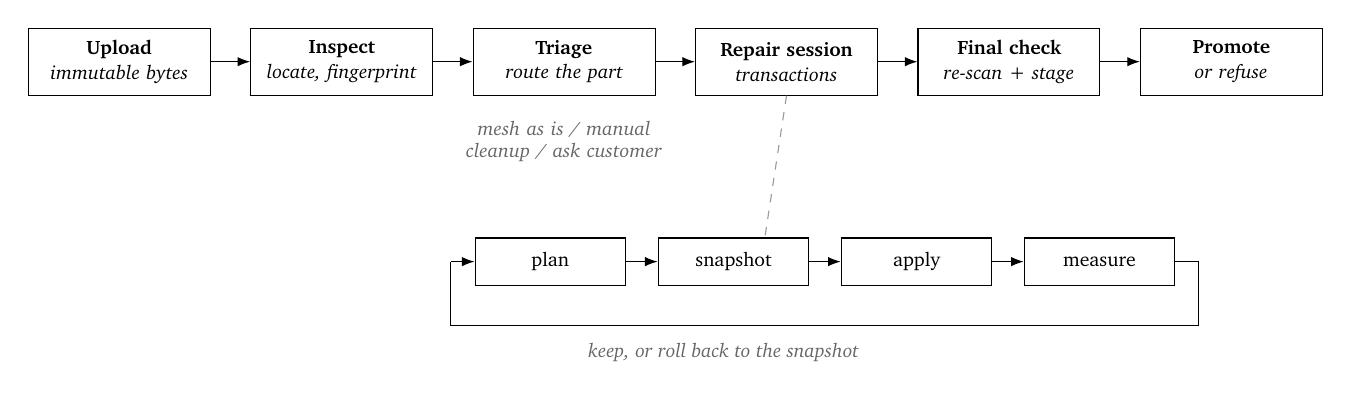
\begin{tikzpicture}[node distance=5mm]
  \node[blk] (up)  {\textbf{Upload}\\[1pt]\scriptsize\itshape immutable bytes};
  \node[blk,right=of up]  (ins) {\textbf{Inspect}\\[1pt]\scriptsize\itshape locate, fingerprint};
  \node[blk,right=of ins] (tri) {\textbf{Triage}\\[1pt]\scriptsize\itshape route the part};
  \node[blk,right=of tri] (ses) {\textbf{Repair session}\\[1pt]\scriptsize\itshape transactions};
  \node[blk,right=of ses] (fin) {\textbf{Final check}\\[1pt]\scriptsize\itshape re-scan + stage};
  \node[blk,right=of fin] (pro) {\textbf{Promote}\\[1pt]\scriptsize\itshape or refuse};
  \foreach \a/\b in {up/ins,ins/tri,tri/ses,ses/fin,fin/pro} \draw[ar] (\a) -- (\b);
  \node[lbl,below=2mm of tri,text width=28mm,align=center]
       {mesh as is / manual cleanup / ask customer};

  \node[sblk,below=18mm of ses,xshift=-30mm] (p1) {plan};
  \node[sblk,right=4mm of p1] (p2) {snapshot};
  \node[sblk,right=4mm of p2] (p3) {apply};
  \node[sblk,right=4mm of p3] (p4) {measure};
  \foreach \a/\b in {p1/p2,p2/p3,p3/p4} \draw[ar] (\a) -- (\b);
  % return path, routed below the row so it crosses nothing
  \coordinate (ra) at ($(p4.east)+(3mm,0)$);
  \coordinate (rb) at ($(p1.west)+(-3mm,0)$);
  \coordinate (rlow) at ($(p1.south)+(0,-5mm)$);
  \draw[thin] (p4.east) -- (ra) -- (ra|-rlow) -- (rb|-rlow) -- (rb);
  \draw[ar] (rb) -- (p1.west);
  \node[lbl,below=1mm of rlow,xshift=22mm] {keep, or roll back to the snapshot};
  \draw[dashed,thin,black!40] (ses.south) -- ($(p2.north)+(4mm,0)$);
\end{tikzpicture}
\caption{The CRS pipeline. Inside the repair session, each operation runs as a transaction against a
snapshot. A candidate that fails any condition from Section~\ref{sec:problem} is rolled back, and
nothing rejected becomes output.}
\label{fig:pipeline}
\end{figure}

\subsection{Inspection and localisation}
The inspector reads the B-rep and reports defects using a deliberately small, stable vocabulary
(Table~\ref{tab:codes}). It keeps facts about the CAD kernel separate from facts about the surface
mesh: a STEP file can be a valid B-rep and still give a bad staged surface, and the report has to
say which layer failed. Each defect is tied to a kernel entity and a fingerprint. When a later
operation rebuilds topology, an entity mapping links old names to new ones and records whether each
link came from the kernel's own history or from geometric matching
(\code{basis: kernel | geometric}), so any downstream credit assignment knows how reliable the link
is.

\begin{table}[t]
\centering
\caption{Defect vocabulary. The kernel codes come from the original design. The \code{mesh\_*} codes
come from the mesh probe (Section~\ref{sec:probe}), have error severity, and are not reserved
judgement codes.}
\label{tab:codes}
\footnotesize\tablecode
\begin{tabularx}{\textwidth}{@{}L{40mm}X@{}}
\toprule
\textbf{Code} & \textbf{Meaning}\\
\midrule
\code{invalid\_brep}            & The OCCT validity check fails.\\
\code{open\_shell}              & A body that must be closed still has free boundaries.\\
\code{wire\_gap}                & Adjacent wire endpoints are disconnected.\\
\code{small\_edge}, \code{small\_face} & An edge length or face area is below the profile threshold.\\
\code{degenerate\_edge}         & An edge is degenerate or nearly zero in length.\\
\code{curve\_inconsistency}     & A 2D or 3D curve is missing or wrong, or same-parameter consistency is broken.\\
\code{self\_intersection}       & A wire or face intersects itself.\\
\code{engine\_staging\_failure} & The selected mesh engine cannot stage the geometry.\\
\code{mesh\_overlapping\_facets}& gmsh reports overlapping facets on a surface.\\
\code{mesh\_edge\_through\_face}& gmsh reports a segment crossing a facet (PLC error).\\
\code{mesh\_open\_loop}         & A face's 1D mesh does not form a closed loop.\\
\code{mesh\_periodic\_surface}  & gmsh cannot mesh a closed, periodic surface.\\
\code{mesh\_no\_volume}, \code{mesh\_timeout} & A solid yields no volume elements, or the probe
exceeds its budget. Both apply to the whole part and are unlocated.\\
\bottomrule
\end{tabularx}
\end{table}

\subsection{Triage}
Triage gives every inspected part one of four routes. A part with no blocking defect goes to
\emph{mesh as is}. A part whose blocking defects all belong to families the catalogue can address
goes to \emph{conservative repair}. A part whose correct fix depends on engineering intent goes to
\emph{manual cleanup}, and one that needs an answer only the customer can give goes to \emph{ask
customer}. Only conservative repair opens a session. One consequence comes up again in
Section~\ref{sec:locate}: a part the inspector calls clean is never scanned further, even if it then
fails to mesh.

\subsection{The operation catalogue}
Each operation implements one protocol. It declares which defect codes it answers and what evidence
it will produce, it can decline before touching the shape, and it returns a candidate together with
its declaration. Table~\ref{tab:ops} lists the catalogue. Apart from the basic connectivity repairs,
every operation sits behind its own deployment flag, and all of those flags are off by default.

\begin{table}[t]
\centering
\caption{The repair catalogue. The OCCT column names the main kernel tool; most operations wrap it
in extra pre- and post-checks. ``Flag'' means the operation is off unless a deployment turns it on.}
\label{tab:ops}
\footnotesize\tablecode
\begin{tabularx}{\textwidth}{@{}L{34mm} L{33mm} X L{15mm}@{}}
\toprule
\textbf{Operation} & \textbf{Answers} & \textbf{Principal OCCT tool} & \textbf{Posture}\\
\midrule
\code{sew\_faces}              & open shells, coincident boundaries      & \code{BRepBuilderAPI\_Sewing} & base\\
\code{fix\_small\_edges}       & small and degenerate edges              & \code{ShapeFix\_Wireframe}         & base\\
\code{fix\_face\_boundary}     & wire ordering, p-curves                 & \code{ShapeFix\_Face}              & base\\
\code{fix\_shape\_global}      & residual validity faults (fallback)     & \code{ShapeFix\_Shape}             & base\\
\code{fix\_small\_faces}       & sub-tolerance slivers                   & \code{ShapeFix\_FixSmallFace}      & flag\\
\code{fill\_planar\_hole}      & bounded planar openings                 & \code{BRepBuilderAPI\_MakeFace} & flag\\
\code{fill\_nonplanar\_hole}   & bounded curved openings                 & \code{BRepFill\_Filling} (G1)      & flag\\
\code{heal\_self\_intersections}& kernel-identified crossings            & \code{ShapeFix\_IntersectionWire} & flag\\
\code{split\_closed\_faces} & \code{mesh\_periodic\_surface}          & \code{ShapeUpgrade\_Shape\-Divide\-Closed} & flag\\
\code{fragment\_bodies}        & \code{mesh\_edge\_through\_face}\newline on assemblies & \code{BOPAlgo\_Builder}      & flag\\
\code{rebuild\_face}           & \code{mesh\_overlapping\_facets}\newline(2D stage) & re-trim from boundary wire & flag; needs reviewer\\
\bottomrule
\end{tabularx}
\end{table}

Three guards protect the operations most likely to change what the part means. First, hole filling
refuses openings wider than 0.75 of the part diagonal, measured across the hole: beyond that the
opening is a missing wall, and a flat lid over a missing wall makes a different part. Second, a
\emph{paired-rim} guard refuses to patch an opening whose rim pairs with another rim to form a
through-passage, because patching both ends would seal a hole the designer intended. Third, face
removal needs an exact face-count declaration and is refused if even one more face disappears.

\subsection{The repair session}\label{sec:session}
The session owns one shape. Before each operation it takes a snapshot by reference. It measures the
candidate (validity, counts, area, volume and tolerances), applies the four conditions from
Section~\ref{sec:problem}, and then either keeps the candidate or restores the snapshot. Every
attempt is written to a run history that records the operation, its target, the declaration, the
measurements and the verdict. A failed or rolled-back attempt is kept as evidence and is never
silently retried on the same aim. When several defects belong to one tangle and so propose the same
heal, the history records the decline once, keyed by aim, rather than once per member face.

We learned to keep instrumentation separate from verdicts, and the lesson came from a failed gate
(Section~\ref{sec:floorgate}). An analyser that only observes, such as a face-crossing scan run
after every operation, can demote outcomes simply by measuring things the baseline never measured.
CRS now runs that scan only at a session's first scan and for the re-inspection that judges a heal.
A crossing that only the analyser sees is reported as \code{analyzer\_only} and does not change the
inspection status, the triage route or how the loop ends.

\subsection{Region-scoped repair}\label{sec:regions}
The original driver re-proved the whole part after every attempt. One local edit triggered a global
proof. That made each iteration expensive, so budgets were kept small: six operations, two stalls
and 120\,s by default. The stall limit applied to the whole run, so two unrelated failures anywhere
ended it. The region-scoped driver (Algorithm~\ref{alg:region}, Figure~\ref{fig:regions}) is built
on one observation. A \emph{region} is a natural unit for four purposes at once: understanding (what
a planner reasons about), verification (a local edit needs only a local proof), reversal (a wrong
hypothesis costs one region instead of the whole run) and cost (regions are independent).

Regions are formed by growing each located defect's bounding box and merging any boxes that
intersect, transitively. The rule deliberately merges too much rather than too little: the members
of a self-intersection tangle all propose the same heal, and splitting the tangle across two regions
would set two packages against the same geometry. Defects with no measurable extent are not merged
with everything else, since that would collapse the part into one region. They go into a single
trailing \emph{unlocated} region, which is flagged, never dropped, and escalated rather than edited.
Regions are visited in order of their most severe defect. An earlier spatial ordering let a run's
clock expire before it reached an error in region 47 of 103.

\begin{algorithm}[t]
\caption{Region-scoped repair. Kernel mutation is serialised; only package authoring may overlap.}
\label{alg:region}
\small
\begin{algorithmic}[1]
\Require upload $U$; budgets $B$ (ops, seconds, attempts per region)
\State $S \gets U$; \quad $D \gets \textsc{WholeShapeScan}(S)$ \Comment{scan 1 of 2}
\State $R \gets \textsc{Decompose}(D)$ \Comment{grown-bbox clustering; unlocated defects form one trailing region}
\ForAll{$r \in R$ ordered by max severity, unlocated last}
  \If{$\neg\, r.\textit{located}$} \State \textsc{Escalate}($r$); \textbf{continue} \EndIf
  \For{$\textit{attempt} \gets 1$ \textbf{to} $B.\textit{attempts}$}
    \State $\textit{pkg} \gets \textsc{Author}(r, D[r], \textit{history}[r])$ \Comment{rules author, or model (Sec.~\ref{sec:model})}
    \If{$\textit{pkg} = \varnothing$} \State \textbf{break} \EndIf
    \State $\textit{snap} \gets \textsc{Snapshot}(S)$
    \State $S' \gets \textsc{Execute}(\textit{pkg}.\textit{plan}, S, \textbf{within } r.\textit{locus})$
    \If{$\textsc{ScopedProof}(S', \textit{pkg}.\textit{predicate}, \textit{caps}(U))
         \wedge \textsc{Review}(\textit{pkg}, \textit{evidence}) = \textsc{accept}$}
      \State $S \gets S'$; \textsc{Commit}($r$); \textbf{break}
    \EndIf
    \State $S \gets \textsc{Restore}(\textit{snap})$;
           $\textit{history}[r].\textsc{append}(\text{measured delta})$ \Comment{fed to the next attempt}
  \EndFor
  \State \textbf{if} no commit \textbf{then} \textsc{Escalate}($r$) \Comment{budget spent: other regions still ship}
\EndFor
\State $D_{\textit{final}} \gets \textsc{WholeShapeScan}(S)$ \Comment{scan 2 of 2; one global verify}
\State \Return $S$, \textsc{Report}($\textit{history}$, $D_{\textit{final}}$)
\end{algorithmic}
\end{algorithm}

\begin{figure}[t]
\centering
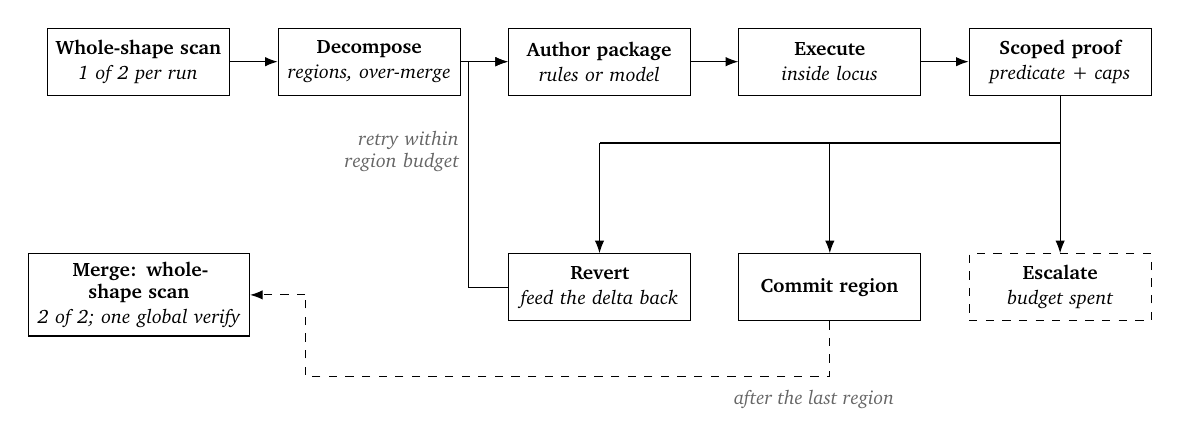
\begin{tikzpicture}[node distance=6mm]
  \node[blk] (scan) {\textbf{Whole-shape scan}\\[1pt]\scriptsize\itshape 1 of 2 per run};
  \node[blk,right=of scan] (dec) {\textbf{Decompose}\\[1pt]\scriptsize\itshape regions, over-merge};
  \node[blk,right=of dec]  (aut) {\textbf{Author package}\\[1pt]\scriptsize\itshape rules or model};
  \node[blk,right=of aut]  (exe) {\textbf{Execute}\\[1pt]\scriptsize\itshape inside locus};
  \node[blk,right=of exe]  (prf) {\textbf{Scoped proof}\\[1pt]\scriptsize\itshape predicate + caps};
  \foreach \a/\b in {scan/dec,dec/aut,aut/exe,exe/prf} \draw[ar] (\a) -- (\b);

  % outcome row
  \node[blk,below=20mm of aut] (rev) {\textbf{Revert}\\[1pt]\scriptsize\itshape feed the delta back};
  \node[blk,below=20mm of exe] (com) {\textbf{Commit region}};
  \node[dblk,below=20mm of prf] (esc) {\textbf{Escalate}\\[1pt]\scriptsize\itshape budget spent};
  % a bus under the proof fans out to the three outcomes, so no line crosses a box
  \coordinate (bus) at ($(prf.south)+(0,-6mm)$);
  \draw[thin] (prf.south) -- (bus);
  \draw[thin] (bus) -- (bus-|rev.north);
  \foreach \n in {rev,com,esc} \draw[ar] (bus-|\n.north) -- (\n.north);

  % retry: the reverted region is authored again
  \draw[ar] (rev.west) -- ++(-5mm,0)
        |- node[lbl,pos=0.3,left,align=right,text width=16mm] {retry within region budget}
        (aut.west);

  % committed regions reach the merge once every region is done
  \node[blk,below=20mm of scan,text width=26mm] (mrg)
       {\textbf{Merge: whole-shape scan}\\[1pt]\scriptsize\itshape 2 of 2; one global verify};
  \coordinate (low) at ($(com.south)+(0,-7mm)$);
  \coordinate (side) at ($(mrg.east)+(7mm,0)$);
  \draw[dashed,thin] (com.south) -- (low) -- (low-|side) -- (side);
  \draw[dashed,ar] (side) -- (mrg.east);
  \node[lbl,below=0.5mm of low,xshift=-2mm] {after the last region};
\end{tikzpicture}
\caption{Control flow of the region driver. A failed predicate or a review rejection reverts only
its own region, and the measured difference goes back to the author. When a region's budget runs out
it escalates while the other regions still commit.}
\label{fig:regions}
\end{figure}

In the target design, kernel mutation remains serialised: the session owns one shape, and OCCT does
not support concurrent mutation of one \code{TopoDS\_Shape}. Only the model calls that author
packages may overlap. The cost saving does not depend on parallelism anyway. It comes from avoided
scans: a run takes two whole-shape scans, one at the start and one at the merge, and in between uses
scoped scans that check only a region's faces. Some invariants are global, such as the paired-rim
guard, and they stay part-wide. An early version checked rims only within one region, so two rims of
the same passage in different regions were both patched and the through-hole was sealed. The corpus
caught this, and it was fixed before merge (Section~\ref{sec:parity}).

\subsection{Target packages and pre-registered predicates}
In the region driver, the unit of action is a \emph{target package}, a scoped work order with five
parts: a \emph{locus} (entity fingerprints and the region they cover), an \emph{intent} in plain
words, a \emph{plan} (an ordered list of catalogue operations within the locus), a
\emph{predicate}, and a \emph{budget}. The predicate states, \emph{before execution}, which
fingerprints will be cleared, which will remain unchanged, and, for mesh defects, which faces will
mesh. The harness then checks that exact claim, so the author cannot grade its own work. It can only
make a claim that something else measures. A claim that names a fingerprint nobody reported fails,
and so does a vacuous claim such as ``the shape is still valid''. A package is also never a cap
waiver: the caps, rollback and progress rule apply to it exactly as they apply to the deterministic
planner.

\subsection{The mesh probe as an inspector}\label{sec:probe}
Meshing a part is the actual goal, and the inspector's defects turned out to be a poor predictor of
meshing failure (Section~\ref{sec:predict}). CRS therefore adds a detector that runs the mesh
itself. The probe uses gmsh 4.15.2~\cite{gmsh}. It imports the shape through gmsh's OCC kernel, sets
\code{MeshSizeMax} to the bounding-box diagonal divided by 40, and generates first the 2D and then
the 3D mesh on one thread, with a 120\,s budget. A part passes if it yields more than zero volume
elements. The probe runs in a freshly exec'd interpreter, never a fork, inside its own process
group, so a gmsh crash or hang cannot take the session with it.

gmsh identifies a failing surface by its tag. The probe imports exactly the shape it is given, so
tags follow that shape's own face map and can be translated into face fingerprints. PLC failures on
assemblies are traced to the pair of bodies in contact. A failure the probe cannot map to an entity
is still reported, as an unlocated defect. If the final whole-part volume mesh fails, the run stops
with the reason \code{unmeshable} and names the bodies. Packages already committed stay committed,
because each one passed its own checks.

A subtle point follows from the fact that gmsh reports only the \emph{first} failure it meets. An
operation that fixes that failure lets the probe go further, and the next failure then appears in
the rescan as if it were new. Treated as new damage, this would roll back an operation exactly where
it worked. That happened in practice: \code{fragment\_bodies} cleared an edge-through-face failure
on one ABC part, and the probe then found overlapping facets on a face that had been failing all
along. CRS therefore treats a new finding as \emph{revealed} rather than \emph{caused} only when all
three of the following hold: the operation answers the mesh code it was aimed at and that defect has
cleared; the new finding is itself a mesh code; and it does not sit on geometry the operation
created, moved or changed. A revealed finding still stays on the defect list, so it blocks a
\code{resolved} ending.

Three operations target the mesh families. \code{split\_closed\_faces} splits periodic faces along
their seams. \code{fragment\_bodies} gives touching bodies a shared, conformal interface while
keeping every body. It declines when bodies interpenetrate, because then there is no safe default
owner for the shared volume. Fusing bodies is deliberately not offered: bodies that touch are often
separate parts on purpose. \code{rebuild\_face} re-trims a single face from its boundary wire. It
acts only on overlaps raised in gmsh's 2D stage, and it must not be enabled for customers until the
reviewer of Section~\ref{sec:model} is live.

\subsection{Model author and semantic reviewer}\label{sec:model}
The region driver accepts any author that maps (region, defects, prior attempts) to a package. A
deterministic \emph{rules author}, which maps each defect code directly to its operation, is the
baseline. A \emph{model author} can fill the same slot. For each region it receives a bounded
observation: the defects with their measurements and gmsh's own error text; each target face's
surface type, area, bounds and neighbours; and what earlier attempts did and why they were undone.
It may reply in one of three ways: with a package; with a verdict that the CAD is sound and the
mesher is the problem; or with a pass. The reply is treated as data, never as code. It is validated
strictly against a schema. A reply that names an operation outside the active catalogue, or a
fingerprint not among the region's defects, is refused before anything runs. A timeout, a parse
failure or a missing model router all produce no package. A ``mesher's problem'' verdict clears
nothing, because if it did it would become an easy way out on hard parts.

There is no numeric ``barely moved'' threshold. The owner chose instead to have each committed
package judged by a \emph{separate} model call with its own prompt. The reviewer is sealed off from
the author. It never sees the author's raw reply, its self-assessment or the observation it read.
The author's intent reaches it only as a field labelled as a claim. What the reviewer does see is
measured: faces, solids, area and volume moved, which faces changed and their neighbours, the
mesh-test result, and a sampled one-sided surface deviation from the pre-package shape (32 points,
using \code{BRepExtrema\_DistShapeShape}). The evidence also states how sparse that sample was. A
measurement that could not be taken appears as the string ``unmeasured'', never as zero, because
zero would read as ``nothing moved''. The verdict is either accept or reject. Unsure counts as
reject, as does no answer, and a rejection reverts the package just as a failed predicate does.
There is no retrying until the reviewer accepts: one rejection buys one more authored attempt, and a
second rejection sends the region to a person. The kernel floor and the declaration accounting
remain hard limits throughout, and the reviewer depends on them to see what actually happened.

\subsection{Configuration posture and audit}
Every capability is controlled by a \code{CAD\_REPAIR\_*} setting that \emph{fails closed}: any
value it does not recognise is read as off, because ``a typo in a deployment must not put a model in
charge of geometry.'' Model-directed features move through the stages \code{off}, \code{shadow} and
\code{live}. In shadow, the model's proposals are recorded next to the run and nothing they contain
is executed. Repaired artefacts are content-addressed, so delivering the same input again writes
identical bytes. The repair report records every observation hash, model reply (clipped), validation
outcome, attempt and review verdict. It serves both as the audit record and as a transition log for
future learning. Appendix~\ref{app:config} lists the settings.

% =============================================================== 5 ==========
\section{The Agentic Loop}\label{sec:v3}

Section~\ref{sec:arch} describes the loop that produced every measurement in this paper. This
section describes what has been built on top of it since. None of it carries a result yet: the
evidence passes are written and have not been run, so everything here is stated as design and as
code that exists, with its status given plainly in Table~\ref{tab:v3status}. The reason for
building it is in Section~\ref{sec:predict} and Section~\ref{sec:corpus}: the deterministic
catalogue's reach is bounded by the geometry it can name, and the families that dominate real
mesh failure are not of that kind.

\subsection{Repair as a job, not a mesher subroutine}\label{sec:goals}

Repair used to be something the meshing pipeline called. It is now a job with a \emph{goal
profile}, and the profile decides only how the run finishes. The loop, the caps, the rollback and
the audit record are the same in all three cases.

\begin{itemize}
  \item \textbf{Standalone.} Clean CAD back to the customer. The finishing verdict is kernel
        validity, one tier-2 meshability reading as a quality score, and semantic review of the
        committed packages. The product mesher is not involved at all.
  \item \textbf{Meshing.} Make the part meshable, then mesh it. The finishing verdict is the name of
        the product mesher; it runs once, at the end, on the winning shape.
  \item \textbf{Benchmark.} Evaluation against the sealed track.
\end{itemize}

A profile also decides what the run reserves. \code{standalone} and \code{benchmark} hold back one
tier-2 hard cap plus its slack so that the finishing reading can actually be taken; \code{meshing}
and an unset profile reserve nothing, which leaves an existing run's deadline byte-for-byte what it
was. A profile never raises: an internal failure is recorded as a profile and an error, so a run
that cannot produce a verdict still reports what it could not do.

\subsection{The cheap-oracle ladder}\label{sec:ladder}

The in-loop question is ``is this part better than it was'', and asking a production mesher is the
wrong way to ask it: the answer is correct and arrives minutes later, on a machine the repair loop
has no business claiming. The ladder (Table~\ref{tab:ladder}) is the set of answers repair may buy.

\begin{table}[h]
\centering
\caption{The verification ladder. Only tiers marked in-loop are reachable from repair. Tier 2's
calibration is the 76/79 agreement of Section~\ref{sec:locate}; tier 2b has no calibration yet.}
\label{tab:ladder}
\footnotesize
\begin{tabularx}{\textwidth}{@{}l L{27mm} l X@{}}
\toprule
\textbf{Tier} & \textbf{Check} & \textbf{In loop} & \textbf{Cost, and what it answers}\\
\midrule
0  & kernel checks          & yes & Milliseconds. Validity, counts, declarations. Every attempt.\\
1  & scoped surface probe   & yes & Sub-second. A region's faces after an edit. Every operation.\\
2  & whole-part coarse mesh & yes & Seconds, hard-capped at 60\,s and $10^6$ elements. One process, coarse sizing, worker CPU. The loop's meshability oracle.\\
2b & tolerant-mesh pass     & yes & Seconds. ``Would the tolerant rung eat this?'' A routing answer for the volume-stage overlap majority.\\
3  & product mesher         & \textbf{no} & Minutes, and a machine. Only when the goal is meshing, only once, on the winner. Never reachable from inside the loop.\\
\bottomrule
\end{tabularx}
\end{table}

\paragraph{The ban is enforced, not promised.}
Tier 3's exclusion is the invariant that keeps a repair
run from quietly becoming a meshing farm, and a comment asking for it would not survive the first
person who needed a better answer in a hurry. The enforcement is a test that parses every module of
the agentic loop and refuses a set of named imports: the machine chooser, the gmsh engine module,
and all but three names of the tetrahedral rung. It reads the syntax tree rather than the file's
text, so a docstring that legitimately mentions a banned name does not trip it and a \emph{deferred}
import inside a function body does not evade it. That second property was proved by mutation: a
function given a lazy import of the machine chooser tripped both guards. A separate guard refuses a
module-level import of gmsh or fTetWild anywhere under the ladder, so neither mesher can be loaded
in the parent process even once.

\paragraph{Tier 2b reports honestly when it cannot run.}
Tier 2b shells out to a coarse tolerant-mesh
pass in a bounded child process, killed by process group at its budget. It has five endings, and
the distinction between them is load-bearing: \code{not\_asked} (the question did not apply),
\code{unavailable} (no binary on this image), \code{no\_answer} (asked, nobody answered in time),
and the two real verdicts. A mutation that collapsed the timeout branch into a refusal was caught
by the suite, which is the point: a part nobody could answer for must not be reported as a part the
rung declined.

\subsection{The grind cost predictor}

Before spending anything on a part, the loop predicts how expensive that part will be to mesh, from
the failure kind and the face count alone. The prediction is a tier --- \code{cheap},
\code{standard}, \code{heavy} or \code{unknown} --- under seven ordered rules: a part nobody
answered for, or one over 1{,}000 faces, is heavy; a part gmsh refused only after building the
whole volume is standard; a surface-stage refusal, or a part that meshed, is cheap. A missing face
count yields \code{unknown}, and so does a probe that was skipped for want of time, since recording
``cheap to mesh'' about a part nobody probed would poison the aggregate it feeds. The predictor
exists so that the investigator's budget is a function of the part rather than a fixed attempt
count, and so that a cheap part cannot buy a heavy part's spend by failing more often.

\subsection{The investigator}\label{sec:investigator}

The one-shot author of Section~\ref{sec:model} gets a bounded observation and must answer with a
finished package. On the live product run it produced 34 proposals and none survived execution.
The machinery held, which was what that run was for, but the shape of the task was wrong: an
engineer handed one photograph of a part does not write the repair either.

The investigator replaces that single turn with a bounded tool loop, one per failing region. Four
tools are declared to the model:

\begin{itemize}
  \item \textbf{look.} Rendered views of the region through the existing review camera.
  \item \textbf{measure.} Distances, a thickness estimate, face properties, body-pair contact.
        Anything the measurement could not establish comes back \texttt{null}, never zero, and the
        thickness figure is labelled an estimate in the field name itself.
  \item \textbf{probe.} Tiers 0 to 2 on a candidate state.
  \item \textbf{edit.} A catalogue operation, applied to a scratch clone.
\end{itemize}

Replies remain data and are validated strictly. Arguments are checked by name: a refusal states the
offending key, the enumeration it violated or the type it was not, and a reference outside its
bounds is refused with the bound named. At most four targets may be named in one call. The whole
observation envelope is clipped to 6\,kB by dropping the longest list and recording that it was
dropped, so a region with a thousand faces does not quietly truncate in the middle of a number.
The two measurements that run kernel Booleans --- common volume and thickness --- run in a bounded
forked child, so a kernel hang cannot take the parent's interpreter with it.

The loop ends, and the endings are the honest ones. The model concludes with a package, with a
verdict that the CAD is sound and the mesher is at fault, or with an escalation naming why the
region needs a person. A model that does not conclude when only proof time remains ends as
\code{budget\_spent}: the clock ended the investigation, and inventing a sixth verdict for that
would dress a timeout as a decision. One record is kept per region and updated in place, so a
second call continues the same investigation rather than reading as two.

\paragraph{Budgets are compute tiers.}
The budget table (Table~\ref{tab:budget}) is indexed by the grind
tier and is not readable from the environment, because a budget is a policy decision measured
offline in the gym rather than a deployment knob. The lookup fails closed in every direction: an
unknown tier, an unrecognised name, a non-string and a predictor that raises all receive the
\emph{smallest} budget.

\begin{table}[h]
\centering
\caption{What one region's investigation may spend. Tool calls are counted, not rounds: a native
round may carry several. A capability answer --- the provider declining tool calls, which falls the
transport back to JSON --- is not charged.}
\label{tab:budget}
\footnotesize
\begin{tabularx}{\textwidth}{@{}l r r r X@{}}
\toprule
\textbf{Grind tier} & \textbf{Tool calls} & \textbf{Model calls} & \textbf{Wall} & \textbf{Typical part}\\
\midrule
\code{cheap}    &  6 &  8 &  60\,s & Surface-stage refusal, or a part the probe already meshes.\\
\code{standard} & 12 & 16 & 150\,s & Refused only after the volume was built.\\
\code{heavy}    & 20 & 26 & 240\,s & No answer at all, or over 1{,}000 faces.\\
\code{unknown}  &  6 &  8 &  60\,s & Nothing measured. Takes the cheap budget by the fail-closed rule.\\
\bottomrule
\end{tabularx}
\end{table}

\paragraph{Native tool calling.}
The model route carries real tool definitions rather than a JSON
protocol described in prose. A provider that declines them is a typed capability answer caught at
the seam, falling the transport back to JSON. The reply cache canonicalises a tool conversation
differently from a text one: call identifiers become first-seen ordinals, because they are noise,
while tool \emph{arguments} and \emph{results} are kept exactly, results by digest. The text
route's scrubbing of long hexadecimal strings and absolute paths would have erased a measured
fingerprint or a face identifier and merged two genuinely different investigations into one cache
entry.

\subsection{The scratch clone}\label{sec:scratch}

An investigator that may edit needs somewhere to edit that is not the part. The scratch session is
a copy of the shape with one structural guard: the first act of an attempt to commit on a scratch
session is to revert and refuse. The guard fires before the predicate is read and before any
review, so there is no ordering of events in which a rehearsal commits.

The isolation is asserted by identity and by kernel topology, not by comparing bytes. This is worth
stating because the obvious test does not work: no kernel operation mutates its input, so the
serialised bytes of ``the clone'' stay identical to the part's even when the clone \emph{is} the
part. The real exposures are tolerance creep through a shared underlying topology and a reset
handing back an already-edited shape, and those are what the assertions name.

A consequence to keep in view: because a scratch session can never reach review, a rehearsal
produces no review signal at all. That an operation was kept is a claim about the operations, not
about whether the result is still the customer's part. Anything learned on a clone still has to
pass review on the real session.

\subsection{Tournament repair}\label{sec:tournament}

One region now gets up to $K$ candidate repair paths rather than one, proposed by the rules author
and by the investigator and deduplicated by a content key over the plan. Each is rehearsed on its
own clone, scored, and the best survivor is \emph{nominated}. Algorithm~\ref{alg:tournament} is the
loop as designed.

\begin{algorithm}[H]
\caption{Tournament repair of one region: rehearse on clones, commit once, review last.}
\label{alg:tournament}
\footnotesize
\begin{algorithmic}[1]
\Require upload $U$; working shape $S$; region $r$ with located defects $D_r$; proposal sources
  $\mathcal{S} = \{\textsc{Rules},\textsc{Investigator}\}$; one region clock $\mathcal{C}$;
  tolerance $\tau$; the customer's deviation threshold $\theta$
\Ensure a committed \emph{and reviewed} package, or an honest refusal
\State $t \gets \textsc{GrindTier}(D_r)$ \Comment{nothing measured $\Rightarrow$ the smallest budget}
\State $w \gets \mathcal{C}.\textsc{RegionWall}(t)$
\If{$w = 0$} \Return \textsc{Refuse}(\code{no\_budget}) \Comment{the budget governs, not an attempt count}
\EndIf
\Statex \textit{propose --- each item names its operation, target fingerprints, claimed defect and declared bound}
\State $\mathcal{K} \gets \textsc{Dedupe}\big(\textstyle\bigcup_{s \in \mathcal{S}} \textsc{Propose}(s, r, D_r)\big)[1{:}K]$
\State \textbf{reject} any item failing its operation's own preconditions \Comment{before it costs an attempt}
\Statex \textit{rehearse --- on copies, so a bad plan costs nothing}
\State $R \gets \varnothing$
\ForAll{$c \in \mathcal{K}$}
  \If{$\mathcal{C}.\textsc{MustConclude}$}
    \State $R \gets R \cup \{\langle c, \textsc{NotRehearsed}\rangle\}$; \textbf{continue}
  \EndIf
  \State $Q \gets \textsc{Clone}(S)$ \Comment{shares no topology with $S$, and cannot commit}
  \For{$i \gets 1$ \textbf{to} $|c.\textit{plan}|$}
    \State $u_i \gets \textsc{Apply}(Q, c.\textit{plan}_i, \tau)$
    \If{$u_i \neq \textsc{Kept}$}
      \State $R \gets R \cup \{\langle c, \textsc{Failed}, \textsc{Reason}(u_i)\rangle\}$; \textbf{break}
    \EndIf
  \EndFor
  \State $v_0 \gets \textsc{Tier}_0(Q)$;\quad $v_1 \gets \textsc{Tier}_1(Q, r)$
  \State $v_2 \gets \textsc{Tier}_2(Q)$ \textbf{if} the region's share exceeds a quarter of the hard cap
  \State $a \gets \textsc{Accounted}(c.\textit{declared}, \textit{measured})$ \Comment{did it do what it said?}
  \State $d \gets \textsc{Deviation}(U, Q, \textsc{EditedFaces}(Q))$ \Comment{against the upload, never the last step}
  \State $\langle \textit{cl}, \textit{rv} \rangle \gets \textsc{DefectDelta}(D_r, Q)$ \Comment{cleared / revealed}
  \State $R \gets R \cup \{\langle c, \textsc{Rehearsed}, v_{0..2}, a, d, \textit{cl}, \textit{rv}\rangle\}$;\quad \textbf{discard} $Q$
\EndFor
\Statex \textit{rank, then commit the winner \emph{once}, on the real shape}
\State $w^\star \gets \textsc{Winner}(R)$ \Comment{rehearsed $>$ not; pass $>$ no-answer $>$ refusal;}
\Statex \hfill \Comment{revealed-none first, then cleared, then deviation, then fewest operations}
\If{$w^\star = \varnothing$} \Return \textsc{Refuse}(\code{no\_candidate\_survived}) \Comment{never promote a loser}
\EndIf
\State $\textit{snap} \gets \textsc{Snapshot}(S)$; apply $w^\star$ under caps and declaration accounting
\Statex \textit{judge --- measurement answered ``did it work''; the model answers ``is it still the part''}
\If{$d \le \theta$ \textbf{and} $a$ \textbf{and} $\textsc{Ops}(w^\star) \cap \textsc{VertexMoving} = \varnothing$}
  \State \textsc{AutoAccept} with audit \Comment{no model call spent}
\Else
  \State $\langle \textit{verdict}, \textit{objection} \rangle \gets \textsc{Review}(\textsc{MeasuredEvidence})$
  \Statex \hfill \Comment{the reviewer reads measurements, never the author's claim}
  \If{$\textit{verdict} \neq \textsc{Accept}$}
    \State $S \gets \textsc{Restore}(\textit{snap})$; return the \emph{measured} objection to the author
    \State \textbf{on a second rejection, escalate to a person} \Comment{no retry-until-accept}
  \EndIf
\EndIf
\State \Return \textit{verdict} \Comment{unsure is reject; a rehearsal win is a nomination, review is the acceptance}
\end{algorithmic}
\end{algorithm}

$K$ defaults to 1 and is clamped to $[1,6]$, so the tournament is inert until a deployment asks for
it and cannot be configured into an unbounded spend. The ordering rules are the part worth arguing
about. A no-answer ranks above a refusal and below a pass, because the three are different facts
and collapsing the first two is the dishonest-ending failure this programme keeps guarding against;
a mutation that ranked a no-answer as a refusal was caught by the ordering table. A revealed defect
outranks any number of cleared ones, so no candidate can buy its way past new damage with volume of
repair. When nothing survives the loop reports that and offers nothing --- there is deliberately no
fall-back to the best-ranked loser.

Rehearsal shares \emph{one} clock per region with the investigation rather than deriving a second,
because two clocks over one deadline is how a region starves the regions after it. Tier 1 is scoped
to the region. Tier 2 is unscoped and is bought only when the candidate's share of the clock
exceeds a quarter of the hard cap; otherwise the rehearsal records \code{no\_time} rather than a
verdict it did not earn.

\subsection{Tiered review and the measured objection}\label{sec:tiered}

The reviewer in Section~\ref{sec:model} reads every committed package, which spends a model call on
changes whose entire story is already in the measurements. Review is now two tiers. A package
auto-accepts, with the audit record written and no model call made, when three things hold: the
measured deviation is under a threshold the customer sets at upload, the declaration fully accounts
for what was measured, and no kept operation is in the vertex-moving set. Everything else goes to
the reviewer. The vertex-moving set is named in one place, and the session-level test pins those
operation names literally --- the first version of that test passed vacuously when the set was
emptied, and a test that cannot fail when the protection is removed is not protecting anything.

Both numeric guards are explicitly guarded against non-finite values. The red run found that an
infinitely negative deviation auto-accepted, and that a not-a-number measurement read as ``fully
accounted''. A float guard on a safety threshold is the kind of hole that never appears on a happy
path.

\paragraph{The objection the author receives is measured.}
A rejection used to be a dead end. It now
returns an objection to the investigator, and the objection is constructed so that the reviewer's
prose has no route to the author. The reviewer names one thing: a \emph{field}, which must be a
member of a closed tuple of fourteen measured evidence keys. That name is then re-fetched from the
tuple rather than copied from the reply, and the value beside it is read from the session's own
evidence. The free-text keys --- the plan, the author's claim, the reviewer's reasons --- are
deliberately not members. A field the evidence does not carry reads \texttt{unmeasured}, never
zero.

The seal is worth describing as a proof rather than an intention, because the first attempt at it
leaked. Trusting the field name from the reply put actual reviewer prose in front of the author in
a test. A second mutation, reading the value from the reply, initially \emph{survived} because the
strict schema happened to neutralise it; the proof was only completed by calling the objection
builder directly, past the schema, which is the level at which a future schema widening would
attack it. On the author's side, the observation handed back on a re-call gains the objection and
nothing else, and the test walks the entire JSON of that observation for every word of a
prose-heavy reviewer reply.

\subsection{The corpus gym}\label{sec:gym}

A prompt change is a policy change, and the only honest way to ship one is to score it offline
against the real-failure corpus first. The gym fingerprints the policy --- twelve declared sources,
among them the prompts, the catalogue text, the budget table and the ladder's constants --- by
parsing each source rather than importing it. Importing the repair stack to read a float would drag
the stack, and on some paths a mesher, into the host gate's process.

Scoring refuses two bundles that do not declare the same stratified sample, naming both hashes. It
reports newly meshed, newly broken, the clean control, a mean score and cost per fixed part,
headline and per stratum, over the intersection of the two arms' rows only. The record ships
\emph{empty} and the gate skips while it is, because seeding a fingerprint from a run nobody
performed would be a fabrication; a test proves the gate turns hard the instant any score lands.
Today no bundle writer records which sample it drew, so the gate refuses every real bundle --- the
gym is built and not yet usable.

\subsection{What is built and what is not}\label{sec:v3status}

\begin{table}[h]
\centering
\caption{Status of the agentic loop. ``Built'' means the module and its tests are merged, each
mutation-proved. It does not mean measured: no evidence pass for any row below has been run, and
every posture flag defaults off.}
\label{tab:v3status}
\footnotesize
\begin{tabularx}{\textwidth}{@{}L{42mm} l X@{}}
\toprule
\textbf{Piece} & \textbf{Built} & \textbf{What is missing}\\
\midrule
Goal profiles                  & yes & The standalone job surface is not wired to an entry point.\\
Oracle ladder, tiers 0--2      & yes & ---\\
Tier 2b tolerant pass          & yes & Reads \code{unavailable} on the pipeline worker image, which carries no tolerant-mesh binary. No calibration.\\
Big-machine import blocklist   & yes & ---\\
Grind predictor                & yes & Predictions are recorded; nothing branches on them yet.\\
Investigator tool loop         & yes & Native tool calling is untested against a real provider; the router test substitutes the transport.\\
Rendered views for \code{look} & no  & The camera seam exists and is unwired.\\
Scratch clone                  & yes & ---\\
Tournament scoring, rehearsal  & yes & \textbf{The winner is not yet committed on the real session.} The nomination is computed and goes nowhere.\\
Tiered review                  & yes & \textbf{Inert.} Nothing declares a deviation threshold, so no package can take the auto-accept tier.\\
Measured review objection      & yes & ---\\
Corpus gym                     & yes & No bundle written today states its sample, so scoring refuses every real bundle.\\
Cross-run outcome memory       & no  & The content-addressed plan key exists as the intended key.\\
Mesher handback into repair    & no  & The named-face refusal is already produced by the meshing ladder.\\
\bottomrule
\end{tabularx}
\end{table}

% =============================================================== 6 ==========
\section{Evaluation Methodology}\label{sec:method}

\subsection{Corpora}
Table~\ref{tab:corpora} lists the corpora. The public ones are pinned by archive and per-file
SHA-256 hashes. No CAD file is committed, since the ABC models~\cite{abc} belong to their creators
and the OCCT dataset has no redistribution licence. Each evidence bundle therefore contains names,
hashes and fetch instructions.

\begin{table}[t]
\centering
\caption{Evaluation corpora.}
\label{tab:corpora}
\small
\begin{tabularx}{\textwidth}{@{}l r L{40mm} >{\raggedright\arraybackslash}X@{}}
\toprule
\textbf{Corpus} & \textbf{Files} & \textbf{Source} & \textbf{Purpose}\\
\midrule
OCCT test dataset 7.8.0    & 331 rows  & Open-Cascade-SAS release V7\_8\_0~\cite{occt} & floor gate for catalogue growth\\
NIST MBE PMI CTC/FTC       & 33        & NIST conformance test files~\cite{nist}       & repair parity, redistributable\\
Generated defect campaign  & 50        & internal defect generator                     & cost of re-inspection\\
Clean references           & 40 of 316 & internal, all 22 part families                & no-op control: nothing may change\\
\code{mesh-failure-real}   & 80        & 33 OCCT + 47 ABC chunk 0050~\cite{abc}        & real files failing a gmsh volume mesh\\
Formula 1000 vehicle body  & 1         & Ludemann Engineering, public~\cite{f1000}     & end-to-end case study\\
\bottomrule
\end{tabularx}
\end{table}

\subsection{Protocol}
Each comparison is a \emph{sealed bundle} made up of a manifest (per-input hash, engine commit,
platform and creation time), the exact settings with their digest, per-file rows, a summary and the
verbatim log. A/B arms run on the same bytes with the same settings except for the one variable
being tested. If the arms ended up differing in more than that, as happened once with the engine
commit (Section~\ref{sec:locate}), the bundle says so and limits its claims accordingly. Settings
are fixed before a run, and no threshold is tuned after the results are seen. Every evidence README
closes with a section titled ``what this does not show''.

Two kinds of control anchor the claims. A \emph{floor gate} requires a flags-on run to repair at
least as many defects as the baseline, with every part kept by the baseline kept again. A \emph{clean
no-op control} runs clean reference parts through the same settings, and any kept operation or any
change in faces, solids or volume counts as a failure. This control catches a kind of damage that
defect counts cannot: an edit to geometry that had nothing wrong with it.

\subsection{Metrics, and one we reject}
We report outcome vectors (\emph{repaired}, \emph{refused}, \emph{nothing to repair}, \emph{not
attempted}, \emph{no change}), counts of kept and rolled-back operations, whole-shape versus scoped
scans, and wall-clock time. For meshing we report \emph{newly meshed} and \emph{newly broken} files,
together with the remaining failures by kind. We do not use the count of runs that end
\emph{resolved} as a repair metric. In a sweep of sliver precision, the number of resolved runs rose
from 17 to 39 while kept operations fell from 32 to 12 and remaining defects rose from 371 to 396.
The setting that resolved the most runs repaired the least, so the count mainly reflects how little
was attempted.

% =============================================================== 6 ==========
\section{Results}\label{sec:results}

\subsection{Case study: a Formula 1000 vehicle body}
We ran CRS on the public Formula 1000 race-car body from Ludemann Engineering~\cite{f1000}, using
the source file as received. The initial inspection reported two invalid-B-rep findings, two
self-intersecting-wire findings, 132 sliver faces and 35 tiny edges. The accepted sequence resolved
the blocking invalidity and removed four measured sliver faces. It left 162 warning-level findings
in place rather than over-defeature the body (Table~\ref{tab:f1000}). On the companion
front-suspension rocker, warnings fell from 12 to 8 and sliver faces from four to one, while the
single solid was preserved and the B-rep stayed valid.

\begin{table}[t]
\centering
\caption{Formula 1000 body, before and after CRS. Staging time is from a single run.}
\label{tab:f1000}
\small
\begin{tabularx}{\textwidth}{@{}l r r X@{}}
\toprule
\textbf{Measure} & \textbf{Before} & \textbf{After} & \textbf{Interpretation}\\
\midrule
OCCT validity     & invalid  & valid         & Error-level topology resolved.\\
Solids            & 8        & 8             & No body lost.\\
Faces             & 421      & 419           & Bounded clean-up; extents unchanged.\\
Findings          & 171      & 162 warnings  & Blocking errors cleared; warnings kept and reported.\\
cfMesh CAD staging& 16.87\,s & 7.99\,s       & Both staged; repaired input about twice as fast here.\\
Surface triangles & 147,545  & 153,117       & The mesher used the repaired topology.\\
\bottomrule
\end{tabularx}
\\[2pt]
\footnotesize This is evidence of repair and mesh-engine readiness on one public model. It is not a
benchmark, and staging is not a completed CFD or FEA solve.
\end{table}

\subsection{Catalogue growth under a floor gate}\label{sec:floorgate}
On the OCCT dataset we compared a baseline against a run with non-planar hole filling and
self-intersection healing switched on. The first flags-on run failed the gate, repairing 318 defects
against the baseline's 430. The cause was the face-crossing scan described in
Section~\ref{sec:session}. Run after every operation, it flagged 19 files with new face-level
crossings, which sent them to manual cleanup, and it rolled back sews on two files (56 defects each)
because of a crossing the baseline had never measured. Once the scan stopped acting as a verdict,
the second run matched the baseline outcome for outcome: 430 repaired defects, 16 promoted files all
passing the final check, no paired-rim file filled, and no cap violated. Because the totals are
equal, we make no claim of improvement. The new heal operation was proposed ten times and declined
all ten, for stated reasons (multi-body inputs, crossings not isolated).

\subsection{Region-scoped driver: parity, cost and the no-op control}\label{sec:parity}
Both drivers ran the same bytes with the same settings, differing only in
\code{CAD\_REPAIR\_REGION\_LOOP} (Tables~\ref{tab:nist} and~\ref{tab:cost}). On NIST the outcome
vectors are identical. The two arms differ in refusal records, 22 against 20, but both refuse the
same 13 distinct rims: the baseline rescans the whole shape every iteration, so after an identity
collision it writes a second record for the same rim. On the generated campaign, whole-shape
re-inspections fell by roughly a factor of ten, and wall-clock time fell even though the region
driver made 802 scoped scans. Across all 40 clean references, neither driver kept a single operation
or changed a single part.

\begin{table}[t]
\centering
\caption{NIST MBE PMI (33 files): repair parity.}
\label{tab:nist}
\small
\begin{tabularx}{\textwidth}{@{}l X l@{}}
\toprule
 & \textbf{Baseline} & \textbf{Region driver}\\
\midrule
Outcomes                           & repaired 7, refused 15, nothing 4, not attempted 6, no change 1 & identical\\
\code{open\_shell} defects repaired& 36                                      & 36\\
Routes                             & conservative 23, manual 6, mesh as is 4 & identical\\
Distinct rims refused              & 13                                      & 13\\
\bottomrule
\end{tabularx}
\end{table}

\begin{table}[t]
\centering
\caption{Generated defect campaign (50 parts) and clean control (40 parts).}
\label{tab:cost}
\small
\begin{tabularx}{\textwidth}{@{}X r r@{}}
\toprule
 & \textbf{Baseline} & \textbf{Region driver}\\
\midrule
Whole-shape re-inspections (campaign)          & 566    & 54\\
Worst case on one part                         & 45     & 2\\
Scoped re-inspections                          & 0      & 802\\
Wall-clock (campaign)                          & 184\,s & 154\,s\\
Per-part verdict                               & ---    & 41 better, 9 tied, 0 worse\\
Clean control: operations kept / parts mutated & 0 / 0  & 0 / 0\\
Clean control: whole-shape scans               & 104    & 40\\
\bottomrule
\end{tabularx}
\end{table}

The cost advantage reverses on fragmented geometry, and any published claim should include both
numbers. NIST CTC-02 used its full 300\,s budget, against the baseline's 96.7\,s. NIST CTC-04, a
637-face part that decomposes into 103 regions, took 43.9\,s against 5.9\,s. The saving holds where
defects cluster and reverses where they are scattered. The comparison also uncovered three defects,
which were fixed before merge: the spatial region walk that never reached an error late in the
order; planner refusals that went unreported on the region path; and the paired-rim guard that
looked only within one region, which let a through-hole be sealed. Unit tests had caught none of the
three.

\subsection{Inspector defects poorly predict mesh failure}\label{sec:predict}
Every NIST file that the inspector flags as \code{open\_shell} meshes in plain gmsh, including one
whose five open shells CRS could not repair. We then assembled 80 public STEP files that genuinely
fail a gmsh volume mesh: 33 from the OCCT 7.8.0 dataset and 47 out of 400 sampled from ABC chunk
0050. Before the mesh-failure work, CRS made only two of them mesh, and for 15 the inspector
reported nothing at all. The failures cluster into a few families (edge through face, overlapping
facets, open loop, periodic surface, no volume, timeout), and none of these appeared in the
inspector's vocabulary at the time. This finding redirected the programme towards measuring
meshability directly.

\subsection{Calibrating the in-loop probe}
In the loop, the probe meshes an in-memory shape. The benchmark, by contrast, scores the delivered
STEP file. We therefore compared the two on all 80 unedited files (Table~\ref{tab:calib}). Our gate
was binary agreement on whether a part meshes. Which failure kind gmsh reports first depends on the
order it processes input, and a STEP round trip can change that order.

\begin{table}[t]
\centering
\caption{Probe calibration: in-loop probe compared with an OCP re-export through STEP.}
\label{tab:calib}
\small
\begin{tabularx}{\textwidth}{@{}X r@{}}
\toprule
\textbf{Measure} & \textbf{Count}\\
\midrule
Binary agreement, in-loop vs re-export                                & 76 of 79 (+1 unreadable)\\
Meshes-vs-fails disagreements (gating; limit 8)                       & 3\\
Both fail, different kind (not gating)                                & 6\\
Reader effect: gmsh reading the upload disagrees with the re-export   & 17 files\\
Rows where a probe reached its 120\,s budget                          & 11\\
\bottomrule
\end{tabularx}
\end{table}

The reader effect is a hazard for any benchmark of this kind. Two files mesh as soon as OCP has read
and re-exported them, so a repair that changes nothing would appear to ``fix'' them. All our meshing
scores use the delivered STEP.

\subsection{Locating mesh failures}\label{sec:locate}
In the first run with the probe live, \textbf{none} of the 15 previously invisible files was
located, against a target of 12. The probe was working. The problem was wiring: triage sends an
inspector-clean file to \emph{mesh as is}, so no session opened and the probe, which runs inside the
session's scan, never ran. That run also differed from its baseline in engine commit, and its bundle
records the confound. Starting a session on every file (a benchmark switch,
\code{-{}-force-repair}) located all 15 of the 15, and raised the number of files with a located
mesh defect from 12 to 74 out of 80. No file that meshed before stopped meshing
(\code{newly\_broken}~$=0$). Five runs now stop as \code{unmeshable} where they previously ended in
a way that concealed the failure.

\subsection{Operations for the mesh-failure families}
With \code{split\_closed\_faces}, \code{fragment\_bodies} and \code{rebuild\_face} enabled and the
model author and reviewer off, we measured the rules baseline on the same 80 files
(Table~\ref{tab:meshops}).

\begin{table}[t]
\centering
\caption{Mesh-failure track (80 files), compared with the location baseline. One pass per arm; the
arms differ in engine commit and in \code{-{}-force-repair}.}
\label{tab:meshops}
\small
\begin{tabularx}{\textwidth}{@{}X r r@{}}
\toprule
 & \textbf{Location baseline} & \textbf{With new operations}\\
\midrule
Meshed before / after              & 1 / 3  & 2 / 5\\
Newly meshed                       & 2      & 3\\
Newly broken                       & 0      & 0\\
Still failing: edge through face   & 25     & 27\\
Still failing: overlapping facets  & 31     & 31\\
Still failing: open loop / periodic& 4 / 3  & 4 / 2\\
Timeouts                           & 10     & 7\\
Stopped \code{unmeshable}          & 5      & 14\\
In-process run seconds             & 4,858  & 9,083\\
\bottomrule
\end{tabularx}
\end{table}

\textbf{None of the three newly meshed files can be credited to a new operation.} The baseline
already meshed two of them without the new operations. On one of those, \code{fragment\_bodies} was
kept, and with a single arm a contribution from it cannot be ruled out completely. The third file
was reached only because forcing a session let the existing \code{fix\_small\_edges} run. Per
operation, \code{fragment\_bodies} was kept on 10 files and rolled back 33 times, and
\code{split\_closed\_faces} ran once and was rolled back. \code{rebuild\_face} never ran.

Two follow-up measurements explain why. An overlap-stage census re-probed the 31 overlapping-facets
files and found that all 31 fail in gmsh's \emph{3D} stage and none in the 2D stage, so
\code{rebuild\_face}, which acts only on 2D-stage overlaps, has nothing to act on in this corpus. A
body-pair census of the 23 multi-solid files with PLC errors tested every pair of bodies whose
bounding boxes meet, using a Boolean common. Eleven files contain at least one overlapping pair and
12 contain only touching pairs. An operation that assumed bodies merely touch would therefore be
wrong on about half of these files, which is why \code{fragment\_bodies} declines on overlap.
Finally, on the two genuine open-loop files the rules author did propose \code{fix\_face\_boundary},
but the targeted faces are already valid closed boundaries. Every relevant \code{ShapeFix\_Wire}
pass reports nothing to do. The 1D-loop failure is something gmsh derives while discretising the
edges, and no wire fixer can see it. We did not add the planned wire passes, because they would have
done nothing.

The clean control, re-sampled across all 22 families, kept zero operations and changed zero parts;
34 of its 40 parts meshed both before and after. The six clean parts that fail the gmsh probe are
themselves a warning about how much weight a single probe failure deserves.

\subsection{The real-failure corpus}\label{sec:corpus}

The 80-file track above is too small to rank a backlog on. We therefore probed 100{,}000 real parts
and kept every one that fails a volume mesh: \textbf{9{,}956 failures, 9.9\% of the parts probed}.
Table~\ref{tab:corpus} is that corpus by family. It is the population every later policy change is
scored against, and it settled three questions the 80-file track could only suggest.

\begin{table}[h]
\centering
\caption{The 9{,}956-file real-failure corpus by family. ``Stage'' is the meshing stage gmsh
refused in; a part is counted once, under the first failure reported. Figures from the committed
harvest aggregate.}
\label{tab:corpus}
\footnotesize
\begin{tabularx}{\textwidth}{@{}l r r r X@{}}
\toprule
\textbf{Family} & \textbf{Files} & \textbf{Surface} & \textbf{Volume} & \textbf{Note}\\
\midrule
Overlapping facets  & 5{,}871 & \textbf{0} & 5{,}840 & 59\% of the corpus. No surface-stage population exists.\\
Edge through face   & 2{,}376 & 0 & 2{,}349 & 982 single-solid, 1{,}394 multi-solid.\\
Timeout             & 587 & 386 & 86 & No answer rather than a verdict.\\
Periodic surface    & 394 & 390 & 1 & The seam-splitting operation's family.\\
Other               & 288 & 9 & 127 & 152 of unknown stage.\\
Open loop           & 227 & 223 & 0 & 94 single-solid, 133 multi-solid.\\
No volume           & 168 & 0 & 167 & 162 single-solid, median 21.5 faces: a tiny-shell family.\\
Crash               & 45 & 33 & 12 & \\
\bottomrule
\end{tabularx}
\end{table}

\paragraph{Face re-trimming has no reach here.}
Of the 5{,}871 overlapping-facet files, \textbf{zero}
fail in the surface stage. \code{rebuild\_face} acts only on surface-stage overlaps, so on this
corpus it has nothing to act on. The 80-file census of Section~\ref{sec:results} suggested this on
31 files; the harvest settles it on 5{,}871. The operation stays in the catalogue for directed use
and is not a line of further investment.

\paragraph{The dominant family is not a CAD-surgery problem.}
5{,}840 volume-stage overlaps are, for the
most part, coincident or self-touching boundaries. The honest answer for them is frequently a
tolerant mesher rather than an edit to the customer's geometry, which is what tier 2b exists to
decide and why its answer is called a \emph{routing} answer rather than a verdict.

\paragraph{Two families are small and specific.}
227 open loops, all surface-stage, are the only
population the bounded vertex-movement operation targets, and how many carry genuine gaps rather
than tolerance-phantom loops is not yet measured. The 168 no-volume files --- 162 of them a single
solid with a median of 21.5 faces --- are a tiny-shell family the harvest found, and whether the
existing sewing and filling operations already repair them is a measurement nobody has taken.

\paragraph{What the deterministic ceiling is.}
The 11-operation catalogue measured a \textbf{8--12\%}
ceiling on the original 80-file track. The programme's target is meshes-after at or above four
times that ceiling on the 9{,}956-file track, with newly-broken held at zero and the clean control
untouched. \textbf{That target is not a result.} The evidence passes that would measure it ---
a tournament evidence run and the held-out measurement pass --- have not been run, and until they
are, this paper reports no agentic gain in either direction.

% =============================================================== 8 ==========
\section{Discussion}\label{sec:discussion}

\paragraph{Measurement-gated editing is safe, but safety is cheap where little is tried.}
Across every controlled run in this paper, no clean part was changed, no cap was violated, and no
file that meshed before stopped meshing. That is what the transactional design is meant to deliver.
Safety is easy to achieve by attempting nothing, though, and the honest headline from the
mesh-failure track is that the main families are largely out of reach of deterministic operations on
real files. 3D-stage overlaps, interpenetrating bodies and open loops that gmsh derives during
discretisation do not yield to local kernel fixes. In our view this is where model judgement has a
legitimate role. Whether two bodies are meant to share an interface, or whether a fault lies in the
CAD or in the mesher, is a semantic question, and the architecture of Section~\ref{sec:model} lets a
model answer it without letting the model grade itself.

\paragraph{Locality is the unifying idea.}
Regions made repair cheaper, but their larger value is that they line up four things that had been
separate: the unit a planner reasons about, the unit that is verified, the unit that is reverted and
the unit that is paid for. The cost reversal on scattered defects marks the limit of the idea. When
defects spread across a hundred regions, per-region attempts multiply faster than the savings from
avoided global scans.

\paragraph{The agentic loop is a bet this paper does not settle.}
Section~\ref{sec:v3} spends the guardrails that Sections~\ref{sec:arch}
and~\ref{sec:results} established. The trade is deliberate and it is a trade: less determinism in
exchange for reach, with safety carried by verification rather than by a small cap on iteration.
Whether the exchange pays is an empirical question and the measurement has not been taken. What we
can say is that the ways it could fail quietly have been closed one at a time, and that most of
them were found by deliberately breaking the code rather than by reading it. A timeout recorded as
a refusal, a no-answer ranked as a refusal, an infinitely negative deviation sailing through an
auto-accept, a not-a-number reading as fully accounted, reviewer prose reaching the author through
a field name, a byte comparison that could not tell a clone from the part it copied: each of those
was a passing test before it was a caught mutation. We report them because a reader's confidence in
the eventual numbers should rest on how the harness behaves when it is wrong, not on the numbers.

\paragraph{The instruments need scrutiny too.}
Several of our results come down to properties of the measuring tools rather than of the geometry.
These include the reader effect, the order in which gmsh reports its first failure, probe failures
on clean parts, a face scan that changed verdicts simply by observing, and a \code{resolved} count
that rewards inaction. Each would have produced a convincing false result had the protocol not
required a control and an explicit statement of what the evidence does not show. We think this
discipline matters more to the credibility of automated CAD repair than any single operation.

% =============================================================== 8 ==========
\section{Limitations and Future Work}\label{sec:limits}

\begin{itemize}
  \item \textbf{Nothing model-directed is yet evaluated.} All results above are from the rules
        baseline, and that remains true of the whole agentic loop of Section~\ref{sec:v3}. The one
        live product run of the model author produced 34 proposals of which 0 survived execution;
        the safety machinery held, and that is the only model-directed result we have. Evaluating
        the agentic path needs two corpus passes that have not been run, on a deployment with a
        model router. Byte-identical replay is retired for agent-driven runs --- a tool
        conversation is not reproducible turn by turn --- and replay now means re-applying the
        recorded packages.
  \item \textbf{The 4x goal is a target, not a measurement.} The programme aims at meshes-after at
        or above four times the deterministic 8--12\% ceiling on the 9{,}956-file track, with
        newly-broken zero and the clean control untouched. No pass has measured any part of it. It
        is stated here so the eventual measurement can be held against it.
  \item \textbf{The agentic loop is not joined end to end.} The tournament computes a winner and
        does not yet commit it on the real session, so its ranking is exercised by its tests and by
        nothing else. Tiered review is inert: no caller declares a per-part deviation threshold, so
        every package still takes the reviewer tier. Both fail safe --- the first offers nothing,
        the second spends a model call it could have saved --- and neither can be described as
        working in a run.
  \item \textbf{Native tool calling has not met a provider.} The investigator's tool transport is
        exercised against a substituted router. Whether the configured provider honours tool calls
        on short non-streaming replies is untested; the JSON fallback exists for the case where it
        does not.
  \item \textbf{Tier 2b cannot answer on the worker image.} The tolerant-mesh pass needs a binary
        the pipeline worker image does not carry, so there every tier-2b question reads
        \code{unavailable}. That is the designed honest answer, and it means the routing answer for
        the corpus's largest family is unavailable exactly where the parts are.
  \item \textbf{Production runs with the agentic loop off.} The posture is committed
        configuration: shared development states the agentic flag live, production states it empty,
        permanently, under a test that executes the configuration step rather than matching its
        text. The loop is therefore unmeasured in production by construction, and the vertex-moving
        operations stay reviewer-gated under every posture value.
  \item \textbf{gmsh is not the product mesher.} The probe gives a quick verdict inside the loop.
        The final verdict belongs to the product's mesh engine, run on the winning candidate. The
        planned production route reverses the direction: when the product mesher fails at named
        faces, it hands that failure back to repair as a request scoped to those faces, within a
        pass budget, so only jobs that fail pay for repair.
  \item \textbf{Single platform, single pass.} All runs were on darwin-arm64 with one gmsh version,
        and run-to-run nondeterminism has not been measured. Some A/B comparisons differ in engine
        commit as well as in the variable under test, and their bundles say so.
  \item \textbf{The generated campaign cannot demonstrate repair.} Its injected defects (thin walls,
        debris, pin holes and the like) lie outside the current catalogue, so it measures only the
        cost of a run.
  \item \textbf{Open policy questions.} These include what licence a model-authored package receives
        on reserved judgement codes, whether a reclassification may persist across uploads (a
        judgement cache keyed by fingerprint would be a cross-tenant channel), and whether ``clean''
        should eventually make warnings block delivery.
\end{itemize}

% =============================================================== 9 ==========
\section{Conclusion}\label{sec:conclusion}

CRS treats CAD repair as a sequence of measured, reversible transactions rather than as a cleanup
filter. That choice has held up under evaluation. Region scoping cut re-inspection cost by about a
factor of ten where defects cluster, with no loss of repair parity and no change to clean parts.
Measuring meshability directly showed that the old defect vocabulary barely predicted what actually
blocks a mesh. The same measurement showed, without ambiguity, that the deterministic catalogue
cannot reach most real mesh failures. A corpus of 9{,}956 real failures harvested from 100{,}000
probed parts then settled which families are worth spending on and which are not.

The next step is built and unmeasured. Model judgement now sits inside the transaction boundary as
a bounded investigation rather than a single proposal: the model looks, measures, probes and edits
on a copy; a tournament of candidates is rehearsed on clones and the best is nominated; the kernel
measures; a separate reviewer, sealed from the author and answering in measurements, decides.
Section~\ref{sec:v3} describes it and Table~\ref{tab:v3status} states what each piece still lacks.
We claim nothing for it yet. Every claim will be checked against the same sealed evidence used
here, scored in the corpus gym before it ships, and reported with its negatives.

% ========================================================== references ======
\begin{thebibliography}{13}
\footnotesize
\bibitem{selfrefine} A. Madaan et al. Self-Refine: Iterative refinement with self-feedback.
  \emph{arXiv:2303.17651}, 2023.
\bibitem{huang} J. Huang et al. Large language models cannot self-correct reasoning yet. In
  \emph{Proc. ICLR}, 2024. arXiv:2310.01798.
\bibitem{mirage} When do agent loops mistake stagnation for progress? \emph{arXiv:2607.25152}, 2026.
\bibitem{ftetwild} Y. Hu, T. Schneider, B. Wang, D. Zorin and D. Panozzo. Fast tetrahedral meshing
  in the wild. \emph{ACM Transactions on Graphics} 39(4), 2020. arXiv:1908.03581.
\bibitem{shewchuk} J. R. Shewchuk. What is a good linear finite element? Interpolation,
  conditioning, anisotropy, and quality measures. In \emph{Proc. 11th International Meshing
  Roundtable}, 2002.
\bibitem{knupp} P. Knupp. Remarks on mesh quality. In \emph{45th AIAA Aerospace Sciences Meeting},
  SAND2007-8128C, 2007.
\bibitem{metaopenfoam} Y. Chen et al. MetaOpenFOAM: An LLM-based multi-agent framework for CFD.
  \emph{arXiv:2407.21320}, 2024.
\bibitem{foamagent} L. Yue et al. Foam-Agent 2.0. \emph{arXiv:2509.18178}, 2025.
\bibitem{abc} S. Koch et al. ABC: A big CAD model dataset for geometric deep learning. In
  \emph{Proc. CVPR}, 2019.
\bibitem{nist} National Institute of Standards and Technology. MBE PMI validation and conformance
  testing: CTC/FTC STEP files, 2024 release.
\bibitem{occt} Open Cascade SAS. Open CASCADE Technology 7.8.0 and test dataset.
  \url{https://github.com/Open-Cascade-SAS/OCCT}.
\bibitem{gmsh} C. Geuzaine and J.-F. Remacle. Gmsh: A 3-D finite element mesh generator with
  built-in pre- and post-processing facilities. \emph{International Journal for Numerical Methods in
  Engineering} 79(11):1309--1331, 2009.
\bibitem{f1000} Ludemann Engineering. Formula 1000 race car design files.
  \url{https://github.com/LudemannEngineering/Formula-1000-Race-Car}. Used under its licence; the
  repaired file is a Hexera-generated modification, and Ludemann Engineering does not endorse Hexera
  or these results.
\end{thebibliography}

% =========================================================== appendices =====
\appendix

\section{Configuration}\label{app:config}
Every setting below fails closed: an unrecognised value is read as the default. The evaluation runs
in Section~\ref{sec:results} raised the run budgets (\code{MAX\_OPS}~$=200$,
\code{STALL\_LIMIT}~$=50$, \code{TIMEOUT\_S}~$=300$, \code{REGION\_ATTEMPTS}~$=6$), and each bundle
records its exact settings.

\begin{table}[h]
\centering
\caption{Principal \code{CAD\_REPAIR\_*} settings and their defaults.}
\label{tab:settings}
\footnotesize\tablecode
\begin{tabularx}{\textwidth}{@{}L{50mm} l X@{}}
\toprule
\textbf{Setting} & \textbf{Default} & \textbf{Role}\\
\midrule
\code{ENABLED}                     & false       & Master switch for repair.\\
\code{MAX\_DEVIATION\_RATIO}       & 0.001       & Surface movement limit as a fraction of the diagonal.\\
\code{MAX\_TOLERANCE\_MM}          & 0.1         & Largest tolerance any sub-shape may carry.\\
\code{MAX\_AREA\_CHANGE\_RATIO}    & 0.02        & Area residual beyond the declaration.\\
\code{MAX\_VOLUME\_CHANGE\_RATIO}  & 0.02        & Volume residual (when solid count does not rise).\\
\code{MAX\_HOLE\_SPAN\_RATIO}      & 0.75        & Widest opening that may be patched.\\
\code{MAX\_OPS} / \code{STALL\_LIMIT} /\newline\code{TIMEOUT\_S} & 6 / 2 / 120 & Run budgets.\\
\code{REGION\_LOOP}                & off         & Region-scoped driver (off, live).\\
\code{REGION\_ATTEMPTS}            & 3           & Authored packages per region.\\
\code{MESH\_PROBE}                 & off         & gmsh probe as inspector and predicate.\\
\code{FILL\_PLANAR\_HOLES}, \code{FILL\_NONPLANAR\_HOLES} & false & Hole filling.\\
\code{FIX\_SMALL\_FACES},\newline\code{HEAL\_SELF\_INTERSECTIONS}& false & Sliver removal; crossing heal.\\
\code{SPLIT\_CLOSED\_FACES},\newline\code{FRAGMENT\_BODIES}      & false & Mesh-family operations.\\
\code{REBUILD\_FACE}               & false       & Face re-trim; needs the reviewer.\\
\code{LLM\_AUTHOR}                 & off         & Model author (off, shadow, live).\\
\code{PACKAGE\_REVIEW}             & off         & Semantic reviewer (off, live).\\
\midrule
\multicolumn{3}{@{}l}{\itshape The agentic loop of Section~\ref{sec:v3}. Every row below is new, and every row is off.}\\
\code{TOLERANT\_PROBE}            & off         & Tier 2b, the tolerant-mesh routing pass (off, live).\\
\code{TOLERANT\_PROBE\_TIMEOUT\_S} & 30         & Must stay below \code{TIMEOUT\_S}, or authoring has no time.\\
\code{INVESTIGATOR}               & off         & The bounded tool loop (off, shadow, live).\\
\code{INVESTIGATOR\_CALL\_TIMEOUT\_S} & 20      & One model call's wall.\\
\code{INVESTIGATOR\_MODEL\_CALLS\_MAX} & 48      & Run-wide ceiling above the per-region budgets.\\
\code{INVESTIGATOR\_REGION\_SHARE} & 0.5        & Largest share of the clock one region may take.\\
\code{INVESTIGATOR\_IMAGES}       & off         & Rendered views on \code{look}; the channel is unwired.\\
\code{TOURNAMENT}                 & off         & Tournament repair (off, live).\\
\code{TOURNAMENT\_K}              & 1           & Candidates per region, clamped to $[1,6]$.\\
\code{AUTO\_ACCEPT}               & off         & The auto-accept review tier; inert without a threshold.\\
\code{REVIEW\_OBJECTION}          & off         & Return the measured objection to the author.\\
\bottomrule
\end{tabularx}
\end{table}

\section{Evidence and Reproduction}
Each result in Section~\ref{sec:results} has a committed evidence directory under
\lcode{devtools/validation/evidence/}, containing its bundle manifest, settings, summary, logs and a
README that states what the evidence does not show. The mesh-failure track's manifest
(\lcode{devtools/validation/corpora/mesh-failure-real.json}) lists every input by name, SHA-256 and
source URL, and the probe-calibration README gives the download and verification steps. Corpus runs
use \lcode{devtools/validation/repair\_corpus.py} with \code{-{}-bundle}. Model-directed runs replay
byte-identically from a recorded-reply cache.

\end{document}
